\setlength{\columnsep}{3pt}
\begin{flushleft}
	\bigskip
	You can create a private software repository that can be used everytime you want to install a package by configuring \textbf{yum server}.
	
	Below are the steps to configure a \textbf{yum server} using \textbf{FTP (file transfer protocol)}:
	
	\begin{enumerate}
		\item First attach the RHEL ISO image to the virtual machine(VM) while the machine is up and running.
		
		\begin{figure}[h!]
			\centering
			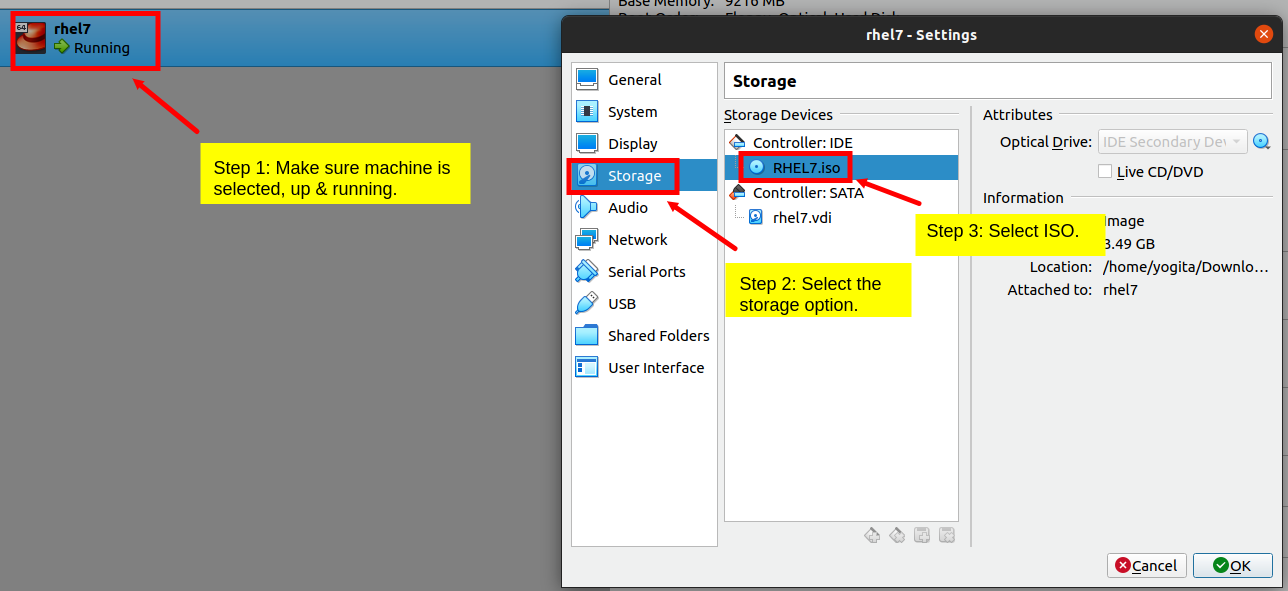
\includegraphics[scale=.3]{content/chapter11/images/ISO.png}
			\caption{Upload RHEL7 ISO}
			\label{fig:iso}
		\end{figure}	
		
		\item Unmount \textbf{/dev/sr0} \& mount the iso image attach on device \textbf{/dev/sr0} to \textbf{"/mnt"} folder.
		\begin{tcolorbox}[breakable,notitle,boxrule=-0pt,colback=black,colframe=black]
			\color{green}
			\fontdimen2\font=9pt
			\# umount	/dev/sr0
			\newline
			\# mount	/dev/sr0	/mnt
			\fontdimen2\font=4pt
		\end{tcolorbox}

		\bigskip
		\item Install following packages from attached ISO image.
		\begin{tcolorbox}[breakable,notitle,boxrule=-0pt,colback=black,colframe=black]
			\color{green}
			\fontdimen2\font=9pt
			\# rpm	-ivh	/mnt/Packages/ftp-xxxx
			\newline
			\# rpm	-ivh 	/mnt/Packages/vsftpd-xxxx
			\newline
			\# rpm	-ivh	/mnt/Packages/createrepo-xxxx
			\fontdimen2\font=4pt
		\end{tcolorbox}
		
		\bigskip
		\item Copy all packages from attached ISO image to pub directory:
		\begin{tcolorbox}[breakable,notitle,boxrule=-0pt,colback=black,colframe=black]
			\color{green}
			\fontdimen2\font=9pt
			\# cp	-rv	/mnt/Packages/*	/var/ftp/pub
			\fontdimen2\font=4pt
		\end{tcolorbox}
		
		\bigskip
		\item Create a repo in pub directory.
		\begin{tcolorbox}[breakable,notitle,boxrule=-0pt,colback=black,colframe=black]
			\color{green}
			\fontdimen2\font=9pt
			\# createrepo	-v	/var/ftp/pub/
			\fontdimen2\font=4pt
		\end{tcolorbox}

		\bigskip
		\item Start and enable the vsftpd service.
		\begin{tcolorbox}[breakable,notitle,boxrule=-0pt,colback=black,colframe=black]
			\color{green}
			\fontdimen2\font=9pt
			\# systemctl   restart   vsftpd
			\newline
			\# systemctl   enable    vsftpd
			\fontdimen2\font=4pt
		\end{tcolorbox}

		\bigskip
		\item Browse the pub directory using browser(like firefox or google chrome) with URL \textbf{ftp://(server IP address)/pub}.
		\newline
		Eg: "ftp://192.168.10.111/pub"

		\bigskip
		\item Create a repository file named \textbf{/etc/yum.repos.d/new.repo}:
		\begin{tcolorbox}[breakable,notitle,boxrule=-0pt,colback=black,colframe=black]
			\color{white}
			\fontdimen2\font=9pt
			[rhcsarepo] \color{yellow}  \# Add title name for this repository 
			\newline
			\color{white}
			name = RHCSA\_REPO
			\color{yellow}
			  \# Add repository name
			\newline
			\color{white}
			enabled = 1
			\newline
			gpgcheck = 0
			\newline
			baseurl = ftp://(server-IP-address)/pub
			\fontdimen2\font=4pt
		\end{tcolorbox}
		\bigskip
		Let's see the parameters of this file in detail.
		
		\newpage
		File explaination:
		
		
		\begin{tabulary}{1.0\textwidth}{|p{10em}|p{14em}|}
			\toprule
			\textbf{Linux OS} & \textbf{Windows OS}\\
			\midrule
			name = RHCSA\_REPO & Set the name of repository \\
			\hline
			enabled = 1 & Defines the state of repository. If value is set to 1 then repository is enabled. If value is set to 0 then repository is disabled. \\
			\hline
			gpgcheck = 0 & Defines whether the integrity of package should be check or not. If value is set to 1, integrity will be checked. If value is set to 0, integrity will not be checked.\\
			\hline
			baseurl = ftp://(server-IP-address)/pub & Defines the location of rpm files \\
			\bottomrule
		\end{tabulary}
		
		
		

		\begin{tcolorbox}[breakable,notitle,boxrule=-0pt,colback=yellow,colframe=yellow]
			\color{black}
			\textbf{Note:} 
			\begin{itemize}
				\item Location of repository file should be \textbf{/etc/yum.repos.d}
				\item Name of the file can be anything
				\item Extension of the file of should be \textbf{".repo"}
			\end{itemize}
		\end{tcolorbox}
		
		


		\item Clean all the cached files from any enabled repository.
		\begin{tcolorbox}[breakable,notitle,boxrule=-0pt,colback=black,colframe=black]
			\color{green}
			\fontdimen2\font=9pt
			\# yum	clean	all
			\fontdimen2\font=4pt
		\end{tcolorbox}
		


		\item Refresh all the enabled repository:
		\begin{tcolorbox}[breakable,notitle,boxrule=-0pt,colback=black,colframe=black]
			\color{green}
			\fontdimen2\font=9pt
			\# yum 	update 	all
			\fontdimen2\font=4pt
		\end{tcolorbox}



		\item Now you can install any packages using the YUM server.
		\newline
		Eg:
		\begin{tcolorbox}[breakable,notitle,boxrule=-0pt,colback=black,colframe=black]
			\color{green}
			\fontdimen2\font=9pt
			\# yum	install	httpd -y		
			\fontdimen2\font=4pt
		\end{tcolorbox}
		

		
		
		
	\end{enumerate}

	

\end{flushleft}
\newpage



